\documentclass[a4paper, 12pt]{article}

\usepackage{hyperref}
\usepackage[warn]{mathtext}
\usepackage[utf8]{inputenc}
\usepackage[T2A]{fontenc}
\usepackage[english,russian]{babel}
\usepackage{multirow}
\usepackage{amsmath,amsfonts,amssymb,amsthm,mathtools}
\usepackage{indentfirst}
\DeclareSymbolFont{T2Aletters}{T2A}{cmr}{m}{it}
\usepackage{ gensymb }
\mathtoolsset{showonlyrefs=true}
\usepackage{euscript}
\usepackage{mathrsfs}
\usepackage[left=2cm,right=2cm,top=2cm,bottom=2cm]{geometry}
\usepackage{graphicx}
\usepackage{wrapfig}
\usepackage[rgb]{xcolor}
\hypersetup{
colorlinks=true,
urlcolor=blue
}


\title{Лабораторная работа}
\author{Гисич Арсений Б03-102}
\date{2022}

\begin{document}

	\begin{center}
		{\large МОСКОВСКИЙ ФИЗИКО-ТЕХНИЧЕСКИЙ ИНСТИТУТ (НАЦИОНАЛЬНЫЙ ИССЛЕДОВАТЕЛЬСКИЙ УНИВЕРСИТЕТ)}
	\end{center}
	\vspace{5 cm}
	{\Large
		\begin{center}
			{\bf Лабораторная работа 3.3.1}\\[0.2 cm]
			Измерение удельного заряда электрона методами магнитной фокусировки и магнетрона
		\end{center}
	}
	\vspace{4 cm}
	\begin{flushright}
		{\Large Выполнил: \\
			\vspace{0.2 cm}
			Гисич Арсений \\
			\vspace{0.2 cm}
			Б03-102 \\}
	\end{flushright}
	\vspace{8 cm}
	\begin{center}
		Долгопрудный\\[0.1 cm]
		2022
	\end{center}
\thispagestyle{empty}

\section{Аннотация}

В данной работе было определено отношение заряда электрона к его массе методами магнитной фокусировки и магнетрона.

\section{Метод магнитной фокусировки}

\subsection{Теоретические сведения}

Здесь удельный заряд электрона определяется по формуле
\begin{equation}\label{eq1}
\dfrac{e}{m_e} = \dfrac{8\pi^2U}{L^2} \left(\dfrac{n^2}{B_{\text{ф}}^2} \right),
\end{equation}
где $U$ --- ускоряющий потенциал в электронной трубке, $L$ --- путь электрона, $B_{\text{ф}}$ --- фокусирующее поле, $n$ --- номер фокуса.

\subsection{Методика измерений}

\begin{wrapfigure}{l}{0.3\textwidth}
  \begin{center}
    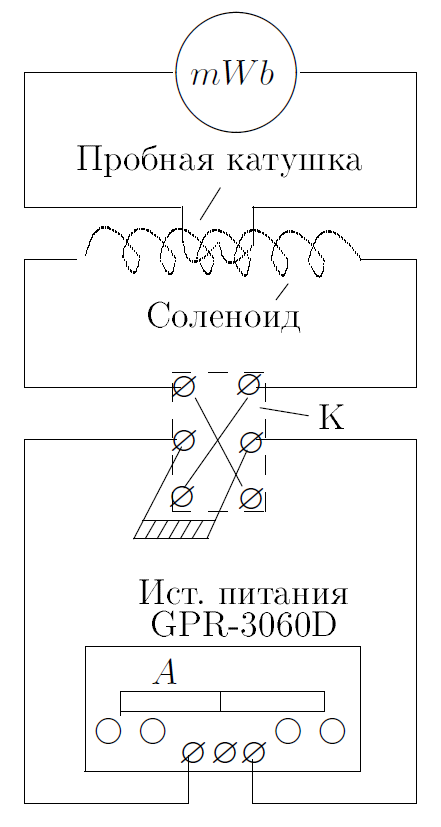
\includegraphics[width = 0.3\textwidth]{1.png}
  \end{center}
  \caption{Схема установки}
  \label{ris1}
\end{wrapfigure}
Основной частью установки является электронный осциллограф, трубка которого вынута и установлена в длинном соленоиде, создающим магнитное поле. Напряжение на отклоняющие пластины и питание подводятся к трубке многожильным кабелем.

Пучок электронов, вылетающих из катода с разными скоростями, ускоряется анодным напряжением. Пропустив пучок сквозь две узкие диафрагмы, можно выделить электроны с практически одинаковой продольной скоростью. Небольшое переменное напряжение, поступающее с клеммы <<Контрольный сигнал>> осциллографа на отклоняющие пластины, изменяет только поперечную составляющую скорости. При увеличении магнитного поля линия на экране стягивается в точку, а затем снова удлиняется. 

Магнитное поле создается постоянным током, величина которого регулируется ручками источника питания и измеряется амперметром. Ключ служит для изменения направления поля в соленоиде.

Величина магнитного поля определяется с помощью милливеберметра.

На точность результатов может влиять внешнее магнитное поле, особенно продольное. 

Измерения магнитного поля с помощью милливеберметра обычно проводятся в предварительных опытах: при отключении ключа устанавливается связь между силой тока и индукцией магнитного поля в соленоиде. 

\subsection{Используемое оборудование}

\begin{enumerate}
    \item электронно-лучевая трубка;
    \item соленоид;
    \item регулируемый источник постоянного тока;
    \item вольтметр;
    \item магнитометр.
\end{enumerate}

\subsection{Результаты измерений и обработка данных}

Параметры установки:
\begin{description}
\item{} $L = 26,5~см$
\item{} $SN = 3000~см^2$
\item{} $U_A = 1,230\pm0,025~кВ$
\end{description}

Результаты измерения калибровочной зависимости $B(I)$ при двух направлениях тока через обмотку представлены в таб.~\ref{tab1}~и~\ref{tab2}.

\begin{table}[h!]
\begin{center}
\begin{tabular}{|c|c|c|c|c|c|}
\hline
$I, A$ & $\sigma_{I}, A$ & $Ф, мВб$ & $\sigma_{Ф}, мВб$ & $B, мТл$ & $\sigma_{B}, мТл$ \\ \hline
0      & 0,005   & 0        & 0,05      & 0        & 0,2       \\ \hline
1,000  & 0,005   & 1,10     & 0,05      & 3,7      & 0,2       \\ \hline
1,500  & 0,005   & 1,60     & 0,05      & 5,3      & 0,2       \\ \hline
2,000  & 0,005   & 2,10     & 0,05      & 7,0      & 0,2       \\ \hline
2,500  & 0,005   & 2,60     & 0,05      & 8,7      & 0,2       \\ \hline
3,000  & 0,005   & 3,10     & 0,05      & 10,3     & 0,2       \\ \hline
3,500  & 0,005   & 3,80     & 0,05      & 12,7     & 0,2       \\ \hline
4,000  & 0,005   & 4,20     & 0,05      & 14,0     & 0,2       \\ \hline
4,500  & 0,005   & 4,50     & 0,05      & 15,0     & 0,2       \\ \hline
\end{tabular}
\end{center}
\caption{Результаты измерений калибровочной кривой при прямом направлении тока}
\label{tab1}
\end{table}

\begin{table}[h!]
\begin{center}
\begin{tabular}{|c|c|c|c|c|c|}
\hline
$I, A$ & $\sigma_{I}, A$ & $Ф, мВб$ & $\sigma_{Ф}, мВб$ & $B, мТл$ & $\sigma_{B}, мТл$ \\ \hline
0      & 0,005   & 0        & 0,05      & 0        & 0,2       \\ \hline
1,000  & 0,005   & 1,00     & 0,05      & 3,3      & 0,2       \\ \hline
1,500  & 0,005   & 1,50     & 0,05      & 5,0      & 0,2       \\ \hline
2,000  & 0,005   & 2,10     & 0,05      & 7,0      & 0,2       \\ \hline
2,500  & 0,005   & 2,70     & 0,05      & 9,0      & 0,2       \\ \hline
3,000  & 0,005   & 3,20     & 0,05      & 10,7     & 0,2       \\ \hline
3,500  & 0,005   & 3,70     & 0,05      & 12,3     & 0,2       \\ \hline
4,000  & 0,005   & 4,40     & 0,05      & 14,7     & 0,2       \\ \hline
4,500  & 0,005   & 4,80     & 0,05      & 16,0     & 0,2       \\ \hline
\end{tabular}
\end{center}
\caption{Результаты измерений калибровочной кривой при обратном направлении тока}
\label{tab2}
\end{table}

Калибровочный график $B(I)$ представлен на рис.~\ref{ris2}.

\begin{figure}[h!]
\begin{flushleft}
    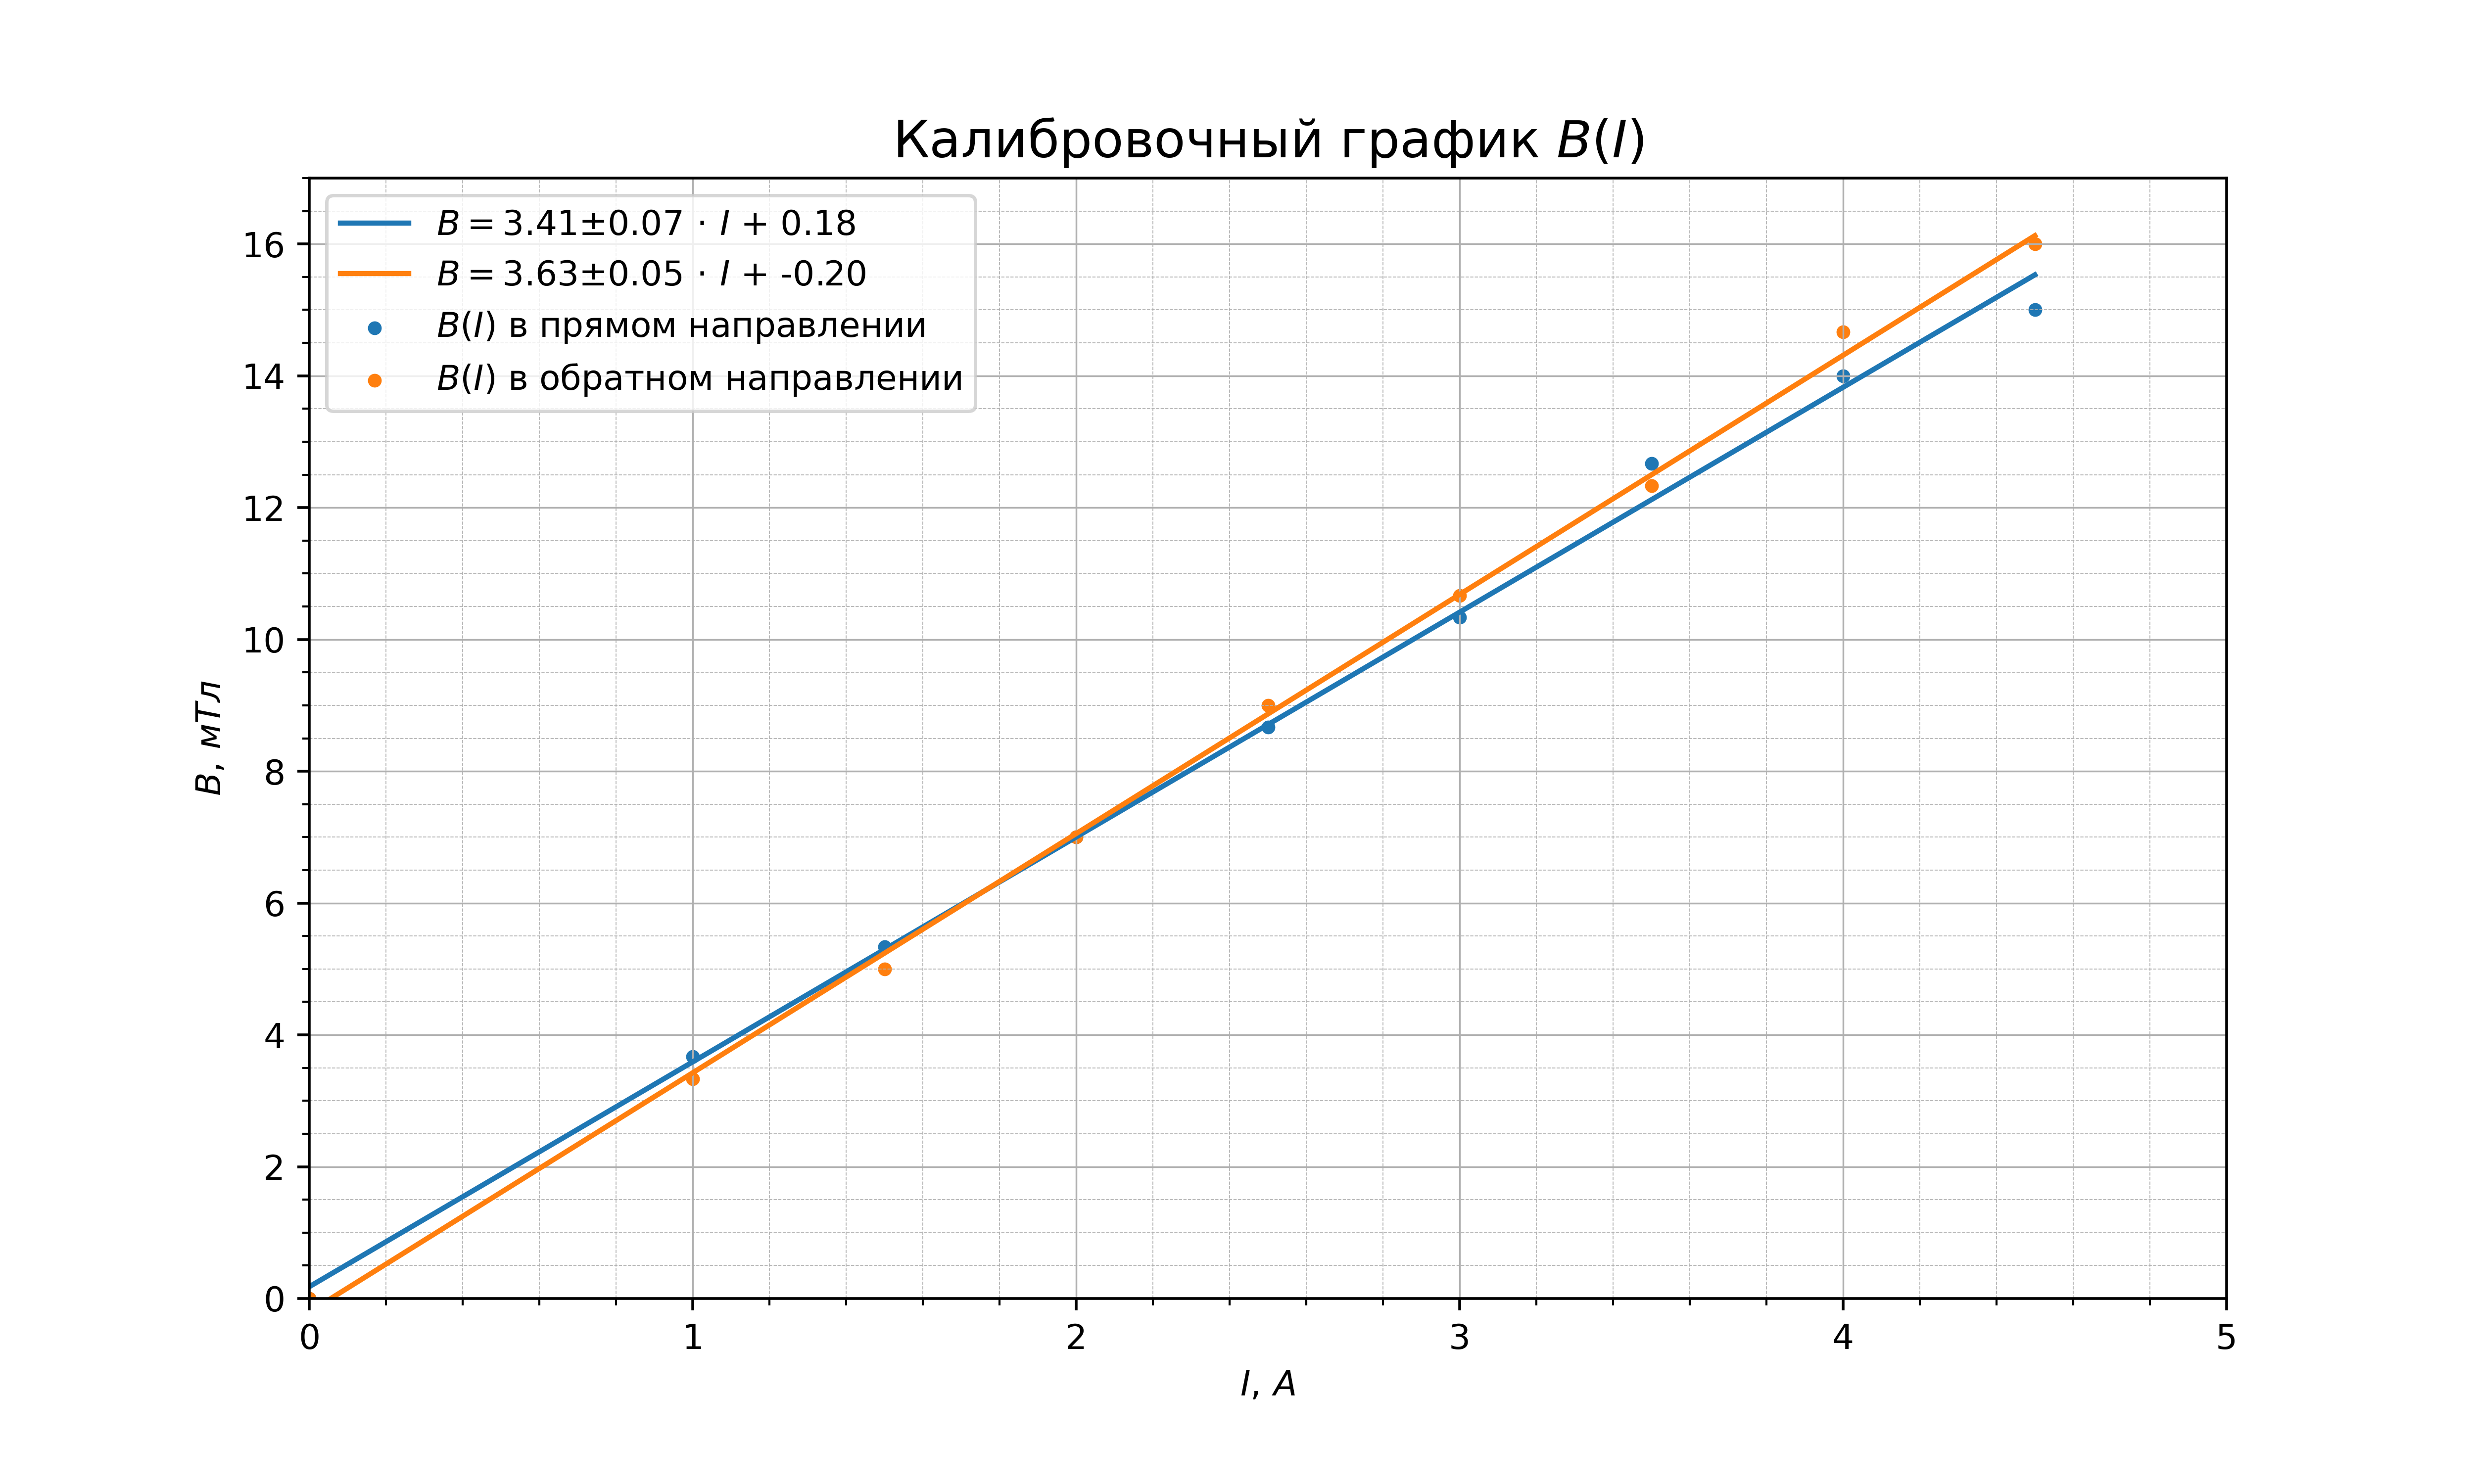
\includegraphics[scale=0.7]{3.3.1_1.png}
\end{flushleft}
\caption{Калибровочный график зависимости магнитного поля в соленоиде от тока в его обмотке}
\label{ris2}
\end{figure}

\vspace{6cm}

Полученные результаты измерения значения $I_ф$ в зависимости от номера фокуса представлены в таб.~\ref{tab3}~и~\ref{tab4}.

\begin{table}[h!]
\begin{center}
\begin{tabular}{|c|c|c|}
\hline
$n$ & $I_ф, A$ & $\sigma_{I_ф}, A$ \\ [0.1cm] \hline
1   & 1,350  & 0,005   \\ \hline
2   & 2,060  & 0,005   \\ \hline
3   & 2,800  & 0,005   \\ \hline
4   & 3,420  & 0,005   \\ \hline
\end{tabular}
\end{center}
\caption{Результаты измерений тока фокусировки при прямом направлении тока}
\label{tab3}
\end{table}

\begin{table}[h!]
\begin{center}
\begin{tabular}{|c|c|c|}
\hline
$n$ & $I_ф, A$ & $\sigma_{I_ф}, A$ \\ [0.1cm] \hline
1   & 1,360  & 0,005   \\ \hline
2   & 2,070  & 0,005   \\ \hline
3   & 2,730  & 0,005   \\ \hline
4   & 3,520  & 0,005   \\ \hline
\end{tabular}
\end{center}
\caption{Результаты измерений тока фокусировки при обратном направлении тока}
\label{tab4}
\end{table}

График зависимости $B_{ф}(n)$ представлен на рис.~\ref{ris3}.

\begin{figure}[h!]
\begin{flushleft}
    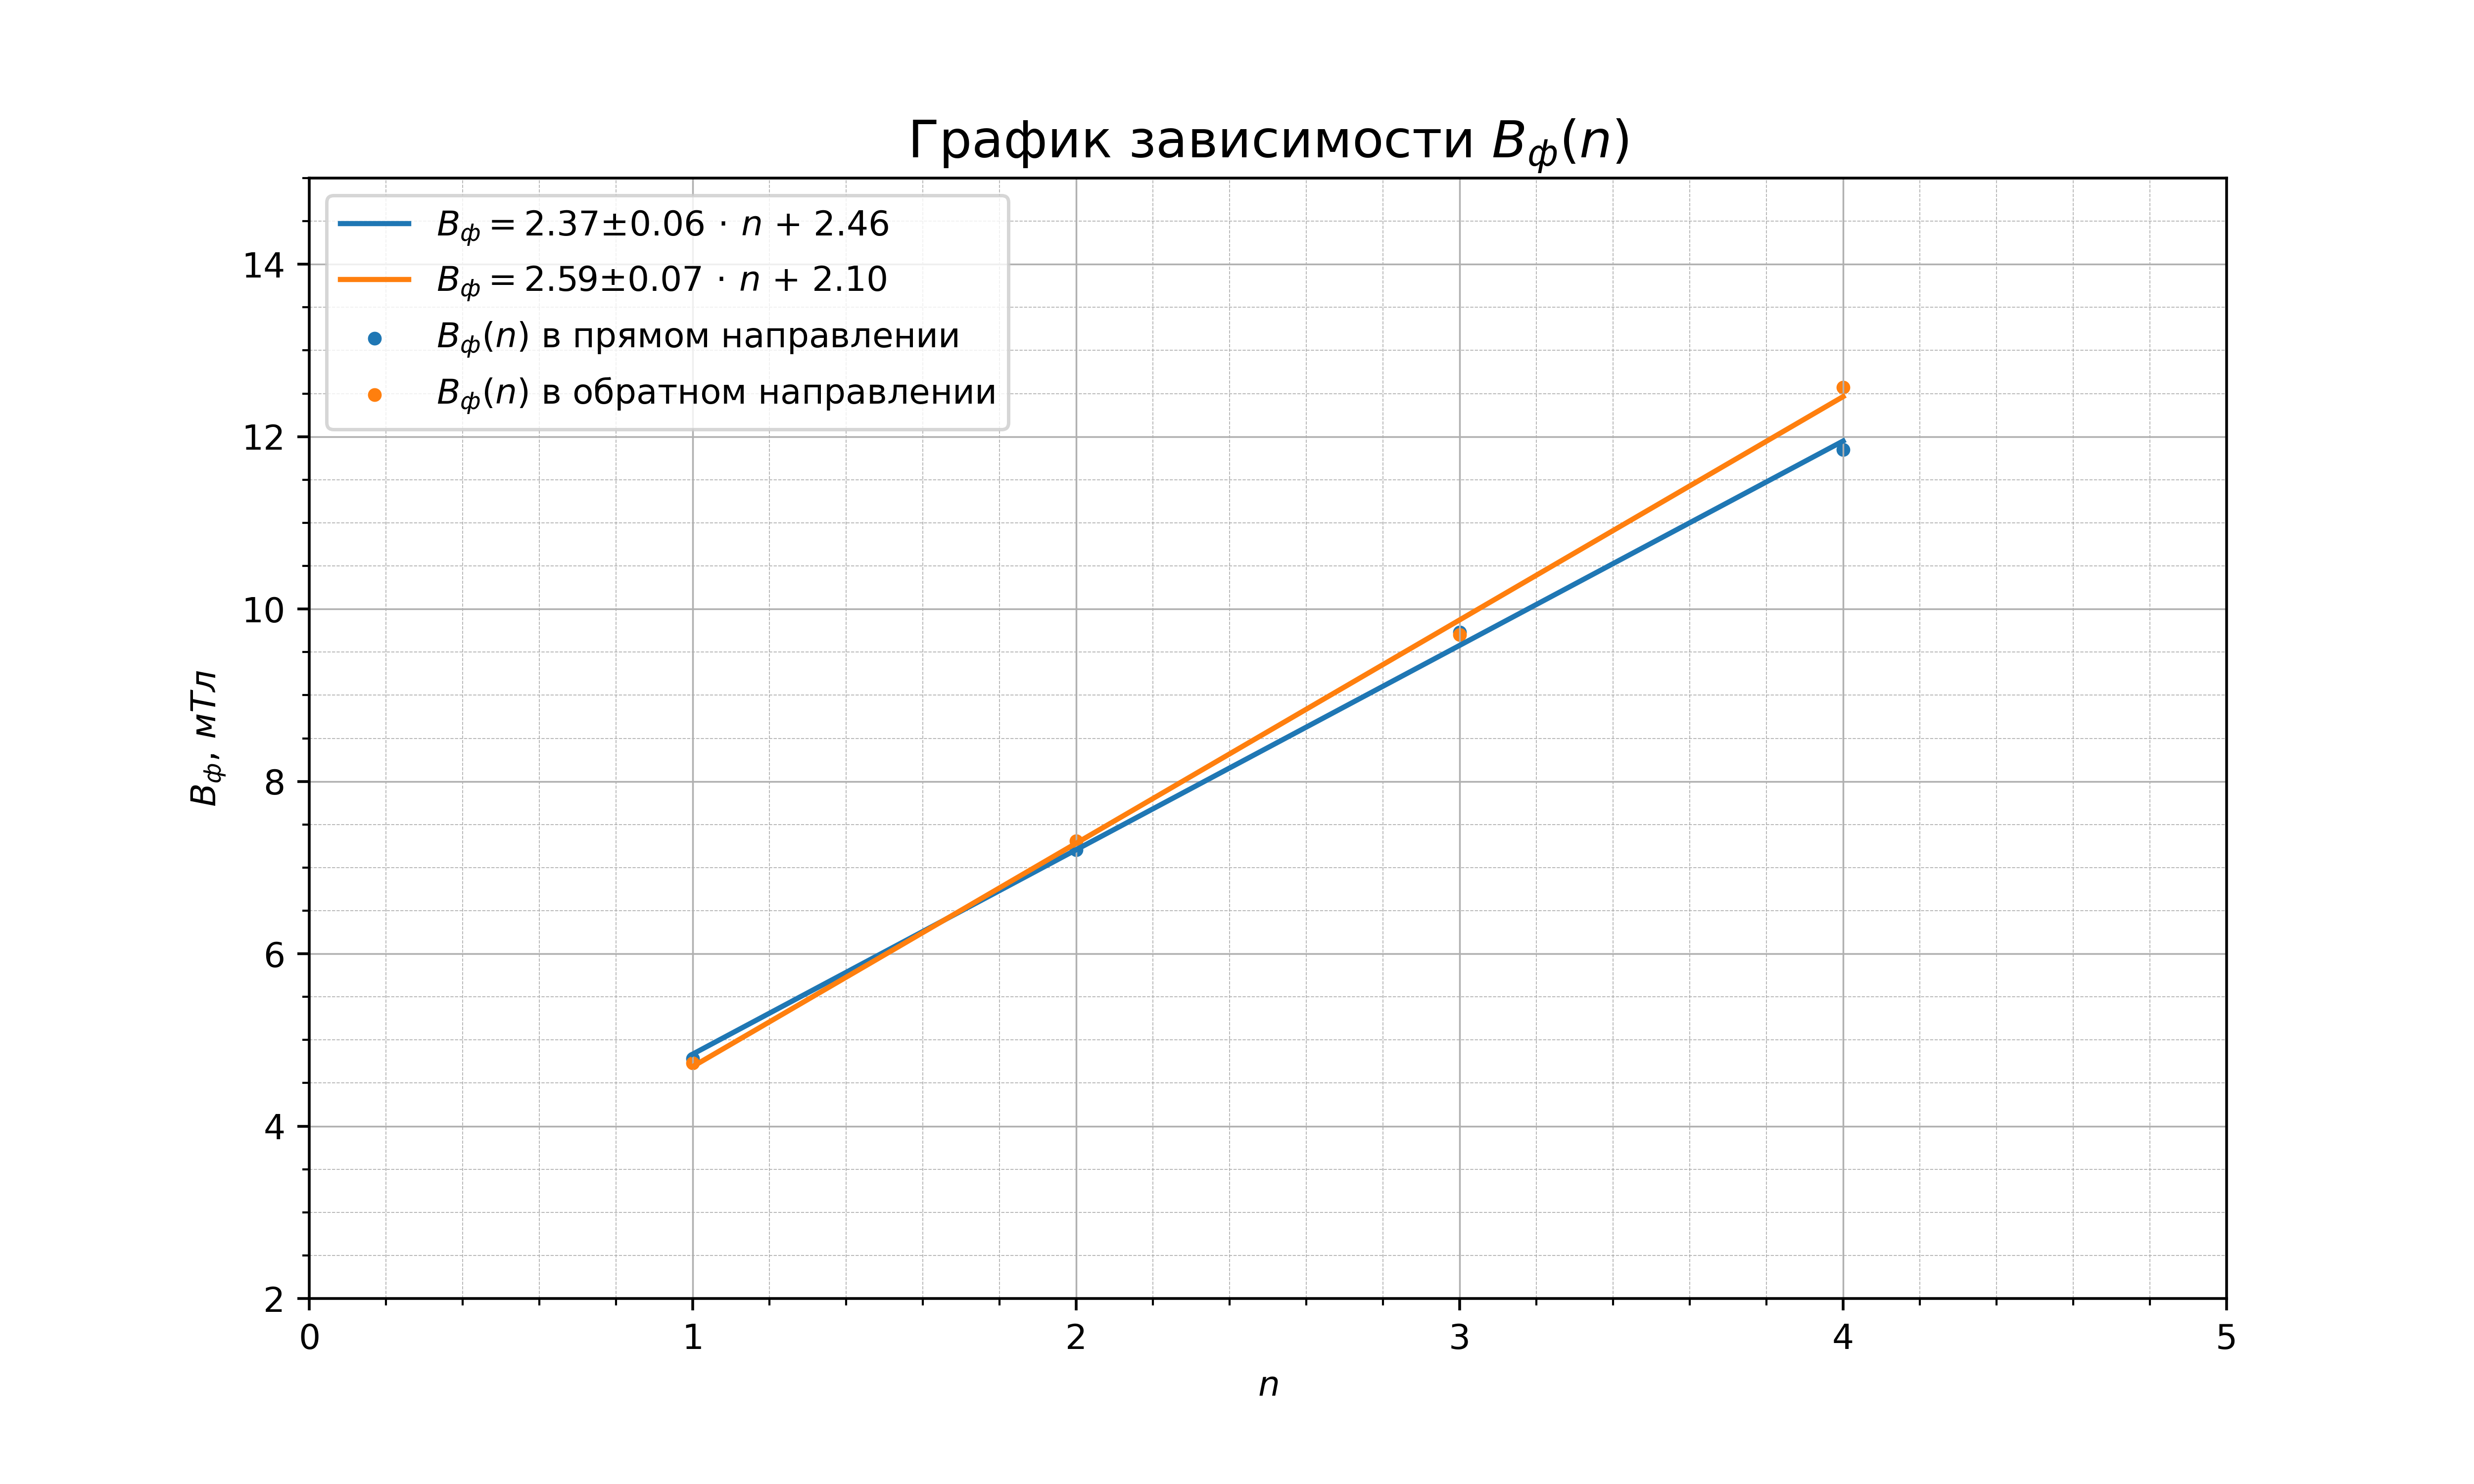
\includegraphics[scale=0.7]{3.3.1_2.png}
\end{flushleft}
\caption{График зависимости фокусирующего поля от номера $n$}
\label{ris3}
\end{figure}

\vspace{3cm}

По формуле \eqref{eq1} вычисляем $e/m$. Полученное значение: $$\frac{e}{m} = 1,6\pm0,1\cdot 10^{11}~Кл/кг.$$

\section{Метод магнетрона}

\subsection{Теоретические сведения}

Здесь удельный заряд электрона определяется по формуле
\begin{equation}\label{eq2}
\dfrac{e}{m_e} = \dfrac{8U_a}{B_{\text{кр}}^2r_a^2},
\end{equation}
где $U_a$ --- анодное напряжение, $B_{\text{кр}}$ --- критическое поле, $r_a$ --- радиус анода.

\subsection{Методика измерений}

Два крайних цилиндра изолированы от среднего небольшими зазорами и используются для устранения краевых эффектов на торцах среднего цилиндра, ток с которого используется при измерениях. В качестве катода используется тонкая вольфрамовая проволока. Катод разогревается переменным током, отбираемым от стабилизированного источника питания. 

С этого же источника на анод лампы подается напряжение, регулируемое с помощью потенциометра и измеряемое вольтметром.

Индукция магнитного поля в соленоиде рассчитывается по току $I_m$, протекающему через обмотку соленоида. Коэффициент пропорциональности между ними указан в установке.

\begin{figure}[h!]
  \begin{center}
    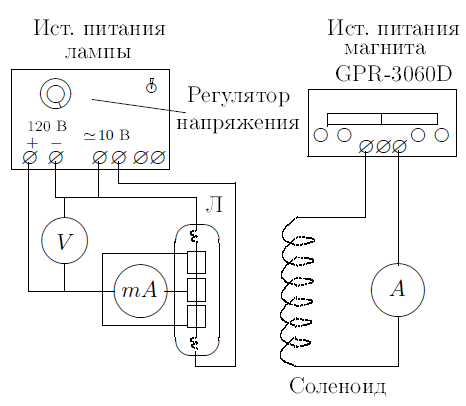
\includegraphics[scale = 1]{2.png}
  \end{center}
  \caption{Схема установки}
  \label{ris4}
\end{figure}

Лампа закреплена в соленоиде. Магнитное поле в соленоиде создается постоянным током, сила которого регулируется ручками источника питания и измеряется амперметром.

\subsection{Используемое оборудование}

\begin{enumerate}
    \item электронная лампа с цилиндрическим анодом;
    \item регулируемый источник постоянного тока;
    \item соленоид;
    \item вольтметр;
    \item 2 амперметра.
\end{enumerate}

\subsection{Результаты измерений и обработка данных}

Параметры установки:
\begin{description}
\item{} $K = 3,5 \cdot 10^{-2}~Tл/A$
\item{} $r_а = 12~мм$
\end{description}

Результаты измерений зависимостей анодного тока от магнитного поля $I_A(B)$ при различных значениях $U_A$ представлены в таб.~\ref{tab5}--\ref{tab10}.

\vspace{5cm}

\begin{table}[h!]
\begin{center}
\begin{tabular}{|c|c|c|c|c|c|}
\hline
$I_C, A$ & $\sigma_{I_C}, A$ & $B, мТл$ & $\sigma_{B}, мТл$ & $I_A, A$ & $\sigma_{I_A}, A$ \\ \hline
0,060 & 0,005  & 2,1    & 0,2     & 0,220 & 0,005  \\ \hline
0,100 & 0,005  & 3,5    & 0,2     & 0,205 & 0,005  \\ \hline
0,110 & 0,005  & 3,9    & 0,2     & 0,210 & 0,005  \\ \hline
0,120 & 0,005  & 4,2    & 0,2     & 0,215 & 0,005  \\ \hline
0,125 & 0,005  & 4,4    & 0,2     & 0,210 & 0,005  \\ \hline
0,130 & 0,005  & 4,6    & 0,2     & 0,055 & 0,005  \\ \hline
0,140 & 0,005  & 4,9    & 0,2     & 0,015 & 0,005  \\ \hline
0,150 & 0,005  & 5,3    & 0,2     & 0,005 & 0,005  \\ \hline
0,160 & 0,005  & 5,6    & 0,2     & 0,003 & 0,005  \\ \hline
0,170 & 0,005  & 6,0    & 0,2     & 0,000 & 0,005  \\ \hline
\end{tabular}
\end{center}
\caption{Результаты измерения $I_A(B)$ при $U_A = 70~B$}
\label{tab5}
\end{table}

\begin{table}[h!]
\begin{center}
\begin{tabular}{|c|c|c|c|c|c|}
\hline
$I_C, A$ & $\sigma_{I_C}, A$ & $B, мТл$ & $\sigma_{B}, мТл$ & $I_A, A$ & $\sigma_{I_A}, A$ \\ \hline
0,060 & 0,005  & 2,1    & 0,2     & 0,225 & 0,005  \\ \hline
0,100 & 0,005  & 3,5    & 0,2     & 0,230 & 0,005  \\ \hline
0,120 & 0,005  & 4,2    & 0,2     & 0,225 & 0,005  \\ \hline
0,130 & 0,005  & 4,6    & 0,2     & 0,220 & 0,005  \\ \hline
0,135 & 0,005  & 4,7    & 0,2     & 0,225 & 0,005  \\ \hline
0,140 & 0,005  & 4,9    & 0,2     & 0,065 & 0,005  \\ \hline
0,145 & 0,005  & 5,1    & 0,2     & 0,030 & 0,005  \\ \hline
0,150 & 0,005  & 5,3    & 0,2     & 0,015 & 0,005  \\ \hline
0,160 & 0,005  & 5,6    & 0,2     & 0,010 & 0,005  \\ \hline
\end{tabular}
\end{center}
\caption{Результаты измерения $I_A(B)$ при $U_A = 80~B$}
\label{tab6}
\end{table}

\begin{table}[h!]
\begin{center}
\begin{tabular}{|c|c|c|c|c|c|}
\hline
$I_C, A$ & $\sigma_{I_C}, A$ & $B, мТл$ & $\sigma_{B}, мТл$ & $I_A, A$ & $\sigma_{I_A}, A$ \\ \hline
0,060 & 0,005  & 2,1    & 0,2     & 0,230 & 0,005  \\ \hline
0,100 & 0,005  & 3,5    & 0,2     & 0,225 & 0,005  \\ \hline
0,120 & 0,005  & 4,2    & 0,2     & 0,225 & 0,005  \\ \hline
0,130 & 0,005  & 4,6    & 0,2     & 0,220 & 0,005  \\ \hline
0,140 & 0,005  & 4,9    & 0,2     & 0,220 & 0,005  \\ \hline
0,145 & 0,005  & 5,1    & 0,2     & 0,090 & 0,005  \\ \hline
0,150 & 0,005  & 5,3    & 0,2     & 0,030 & 0,005  \\ \hline
0,160 & 0,005  & 5,6    & 0,2     & 0,010 & 0,005  \\ \hline
0,170 & 0,005  & 6,0    & 0,2     & 0,000 & 0,005  \\ \hline
\end{tabular}
\end{center}
\caption{Результаты измерения $I_A(B)$ при $U_A = 90~B$}
\label{tab7}
\end{table}

\begin{table}[h!]
\begin{center}
\begin{tabular}{|c|c|c|c|c|c|}
\hline
$I_C, A$ & $\sigma_{I_C}, A$ & $B, мТл$ & $\sigma_{B}, мТл$ & $I_A, A$ & $\sigma_{I_A}, A$ \\ \hline
0,050 & 0,005  & 1,8    & 0,2     & 0,230 & 0,005  \\ \hline
0,100 & 0,005  & 3,5    & 0,2     & 0,225 & 0,005  \\ \hline
0,120 & 0,005  & 4,2    & 0,2     & 0,230 & 0,005  \\ \hline
0,130 & 0,005  & 4,6    & 0,2     & 0,230 & 0,005  \\ \hline
0,140 & 0,005  & 4,9    & 0,2     & 0,225 & 0,005  \\ \hline
0,145 & 0,005  & 5,1    & 0,2     & 0,225 & 0,005  \\ \hline
0,150 & 0,005  & 5,3    & 0,2     & 0,115 & 0,005  \\ \hline
0,155 & 0,005  & 5,4    & 0,2     & 0,050 & 0,005  \\ \hline
0,160 & 0,005  & 5,6    & 0,2     & 0,025 & 0,005  \\ \hline
0,170 & 0,005  & 6,0    & 0,2     & 0,010 & 0,005  \\ \hline
0,180 & 0,005  & 6,3    & 0,2     & 0,005 & 0,005  \\ \hline
\end{tabular}
\end{center}
\caption{Результаты измерения $I_A(B)$ при $U_A = 100~B$}
\label{tab8}
\end{table}

\begin{table}[h!]
\begin{center}
\begin{tabular}{|c|c|c|c|c|c|}
\hline
$I_C, A$ & $\sigma_{I_C}, A$ & $B, мТл$ & $\sigma_{B}, мТл$ & $I_A, A$ & $\sigma_{I_A}, A$ \\ \hline
0,060 & 0,005  & 2,1    & 0,2     & 0,230 & 0,005  \\ \hline
0,100 & 0,005  & 3,5    & 0,2     & 0,230 & 0,005  \\ \hline
0,120 & 0,005  & 4,2    & 0,2     & 0,225 & 0,005  \\ \hline
0,150 & 0,005  & 5,3    & 0,2     & 0,225 & 0,005  \\ \hline
0,160 & 0,005  & 5,6    & 0,2     & 0,090 & 0,005  \\ \hline
0,165 & 0,005  & 5,8    & 0,2     & 0,040 & 0,005  \\ \hline
0,170 & 0,005  & 6,0    & 0,2     & 0,025 & 0,005  \\ \hline
0,180 & 0,005  & 6,3    & 0,2     & 0,010 & 0,005  \\ \hline
0,190 & 0,005  & 6,7    & 0,2     & 0,005 & 0,005  \\ \hline
\end{tabular}
\end{center}
\caption{Результаты измерения $I_A(B)$ при $U_A = 110~B$}
\label{tab9}
\end{table}

\begin{table}[h!]
\begin{center}
\begin{tabular}{|c|c|c|c|c|c|}
\hline
$I_C, A$ & $\sigma_{I_C}, A$ & $B, мТл$ & $\sigma_{B}, мТл$ & $I_A, A$ & $\sigma_{I_A}, A$ \\ \hline
0,060 & 0,005 & 2,1 & 0,2 & 0,230 & 0,005 \\ \hline
0,100 & 0,005 & 3,5 & 0,2 & 0,230 & 0,005 \\ \hline
0,150 & 0,005 & 5,3 & 0,2 & 0,225 & 0,005 \\ \hline
0,160 & 0,005 & 5,6 & 0,2 & 0,225 & 0,005 \\ \hline
0,165 & 0,005 & 5,8 & 0,2 & 0,095 & 0,005 \\ \hline
0,170 & 0,005 & 6,0 & 0,2 & 0,055 & 0,005 \\ \hline
0,180 & 0,005 & 6,3 & 0,2 & 0,015 & 0,005 \\ \hline
0,190 & 0,005 & 6,7 & 0,2 & 0,010 & 0,005 \\ \hline
0,200 & 0,005 & 7,0 & 0,2 & 0,005 & 0,005 \\ \hline
\end{tabular}
\end{center}
\caption{Результаты измерения $I_A(B)$ при $U_A = 120~B$}
\label{tab10}
\end{table}

График зависимостей анодного тока от магнитного поля $I_A(B)$ при различных значениях $U_A$ представлен на рис.~\ref{ris5}.

\vspace{5cm}

\begin{figure}[h!]
\begin{flushleft}
    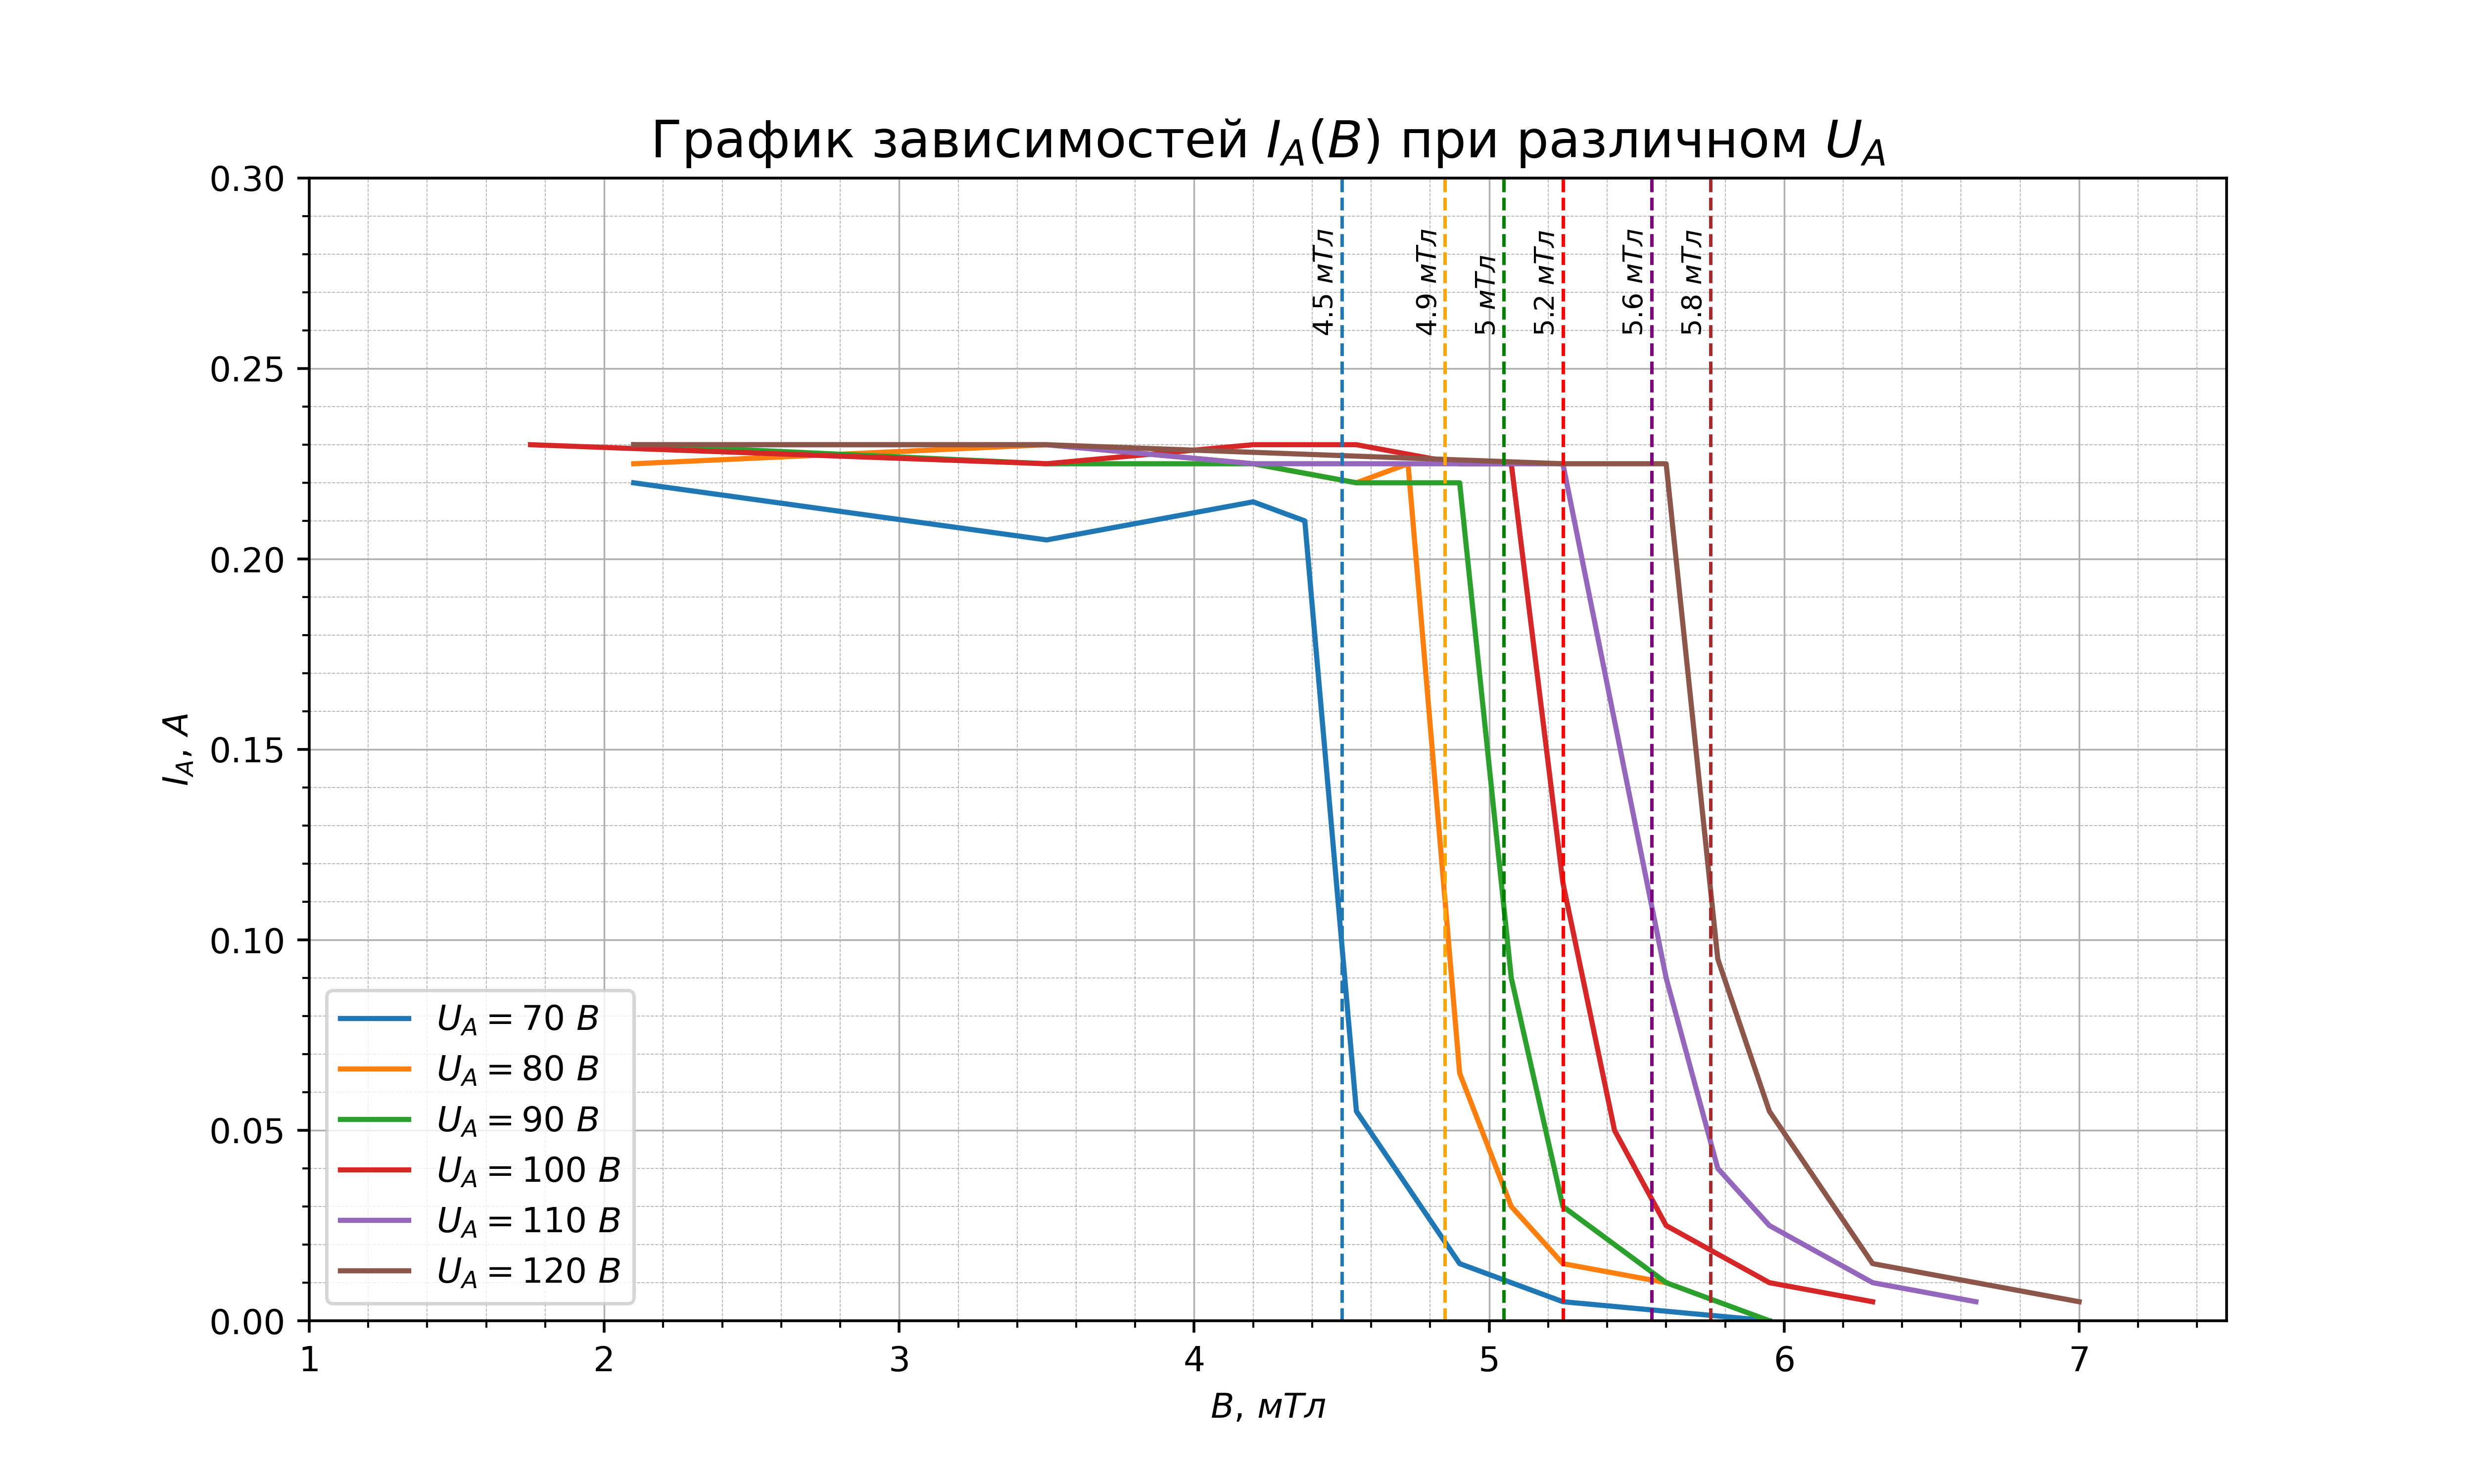
\includegraphics[scale=0.7]{3.3.1_3.png}
\end{flushleft}
\caption{Семейство зависимостей анодного тока от магнитного поля $I_A(B)$ при различных значениях $U_A$}
\label{ris5}
\end{figure}

Полученные критические значения индукции магнитного поля $B_{кр}$ при различных значениях $U_A$ представлены в таб.~\ref{tab11}.

\vspace{5cm}

\begin{table}[h!]
\begin{center}
\begin{tabular}{|c|c|c|}
\hline
$U_A, B$ & $B_{кр}, мТл$ & $\sigma_{B_{кр}}, мТл$ \\ \hline
70 & 4,5 & 0,1 \\ \hline
80 & 4,9 & 0,1 \\ \hline
90 & 5,0 & 0,1 \\ \hline
100 & 5,2 & 0,1 \\ \hline
110 & 5,6 & 0,1 \\ \hline
120 & 5,8 & 0,1 \\ \hline
\end{tabular}
\end{center}
\caption{Полученная зависимость $B_{кр}(U_A)$}
\label{tab11}
\end{table}

Полученный график зависимости $B^2_{кр}(U_A)$ представлен на рис.~\ref{ris6}.

\vspace{10cm}

\begin{figure}[h!]
\begin{flushleft}
    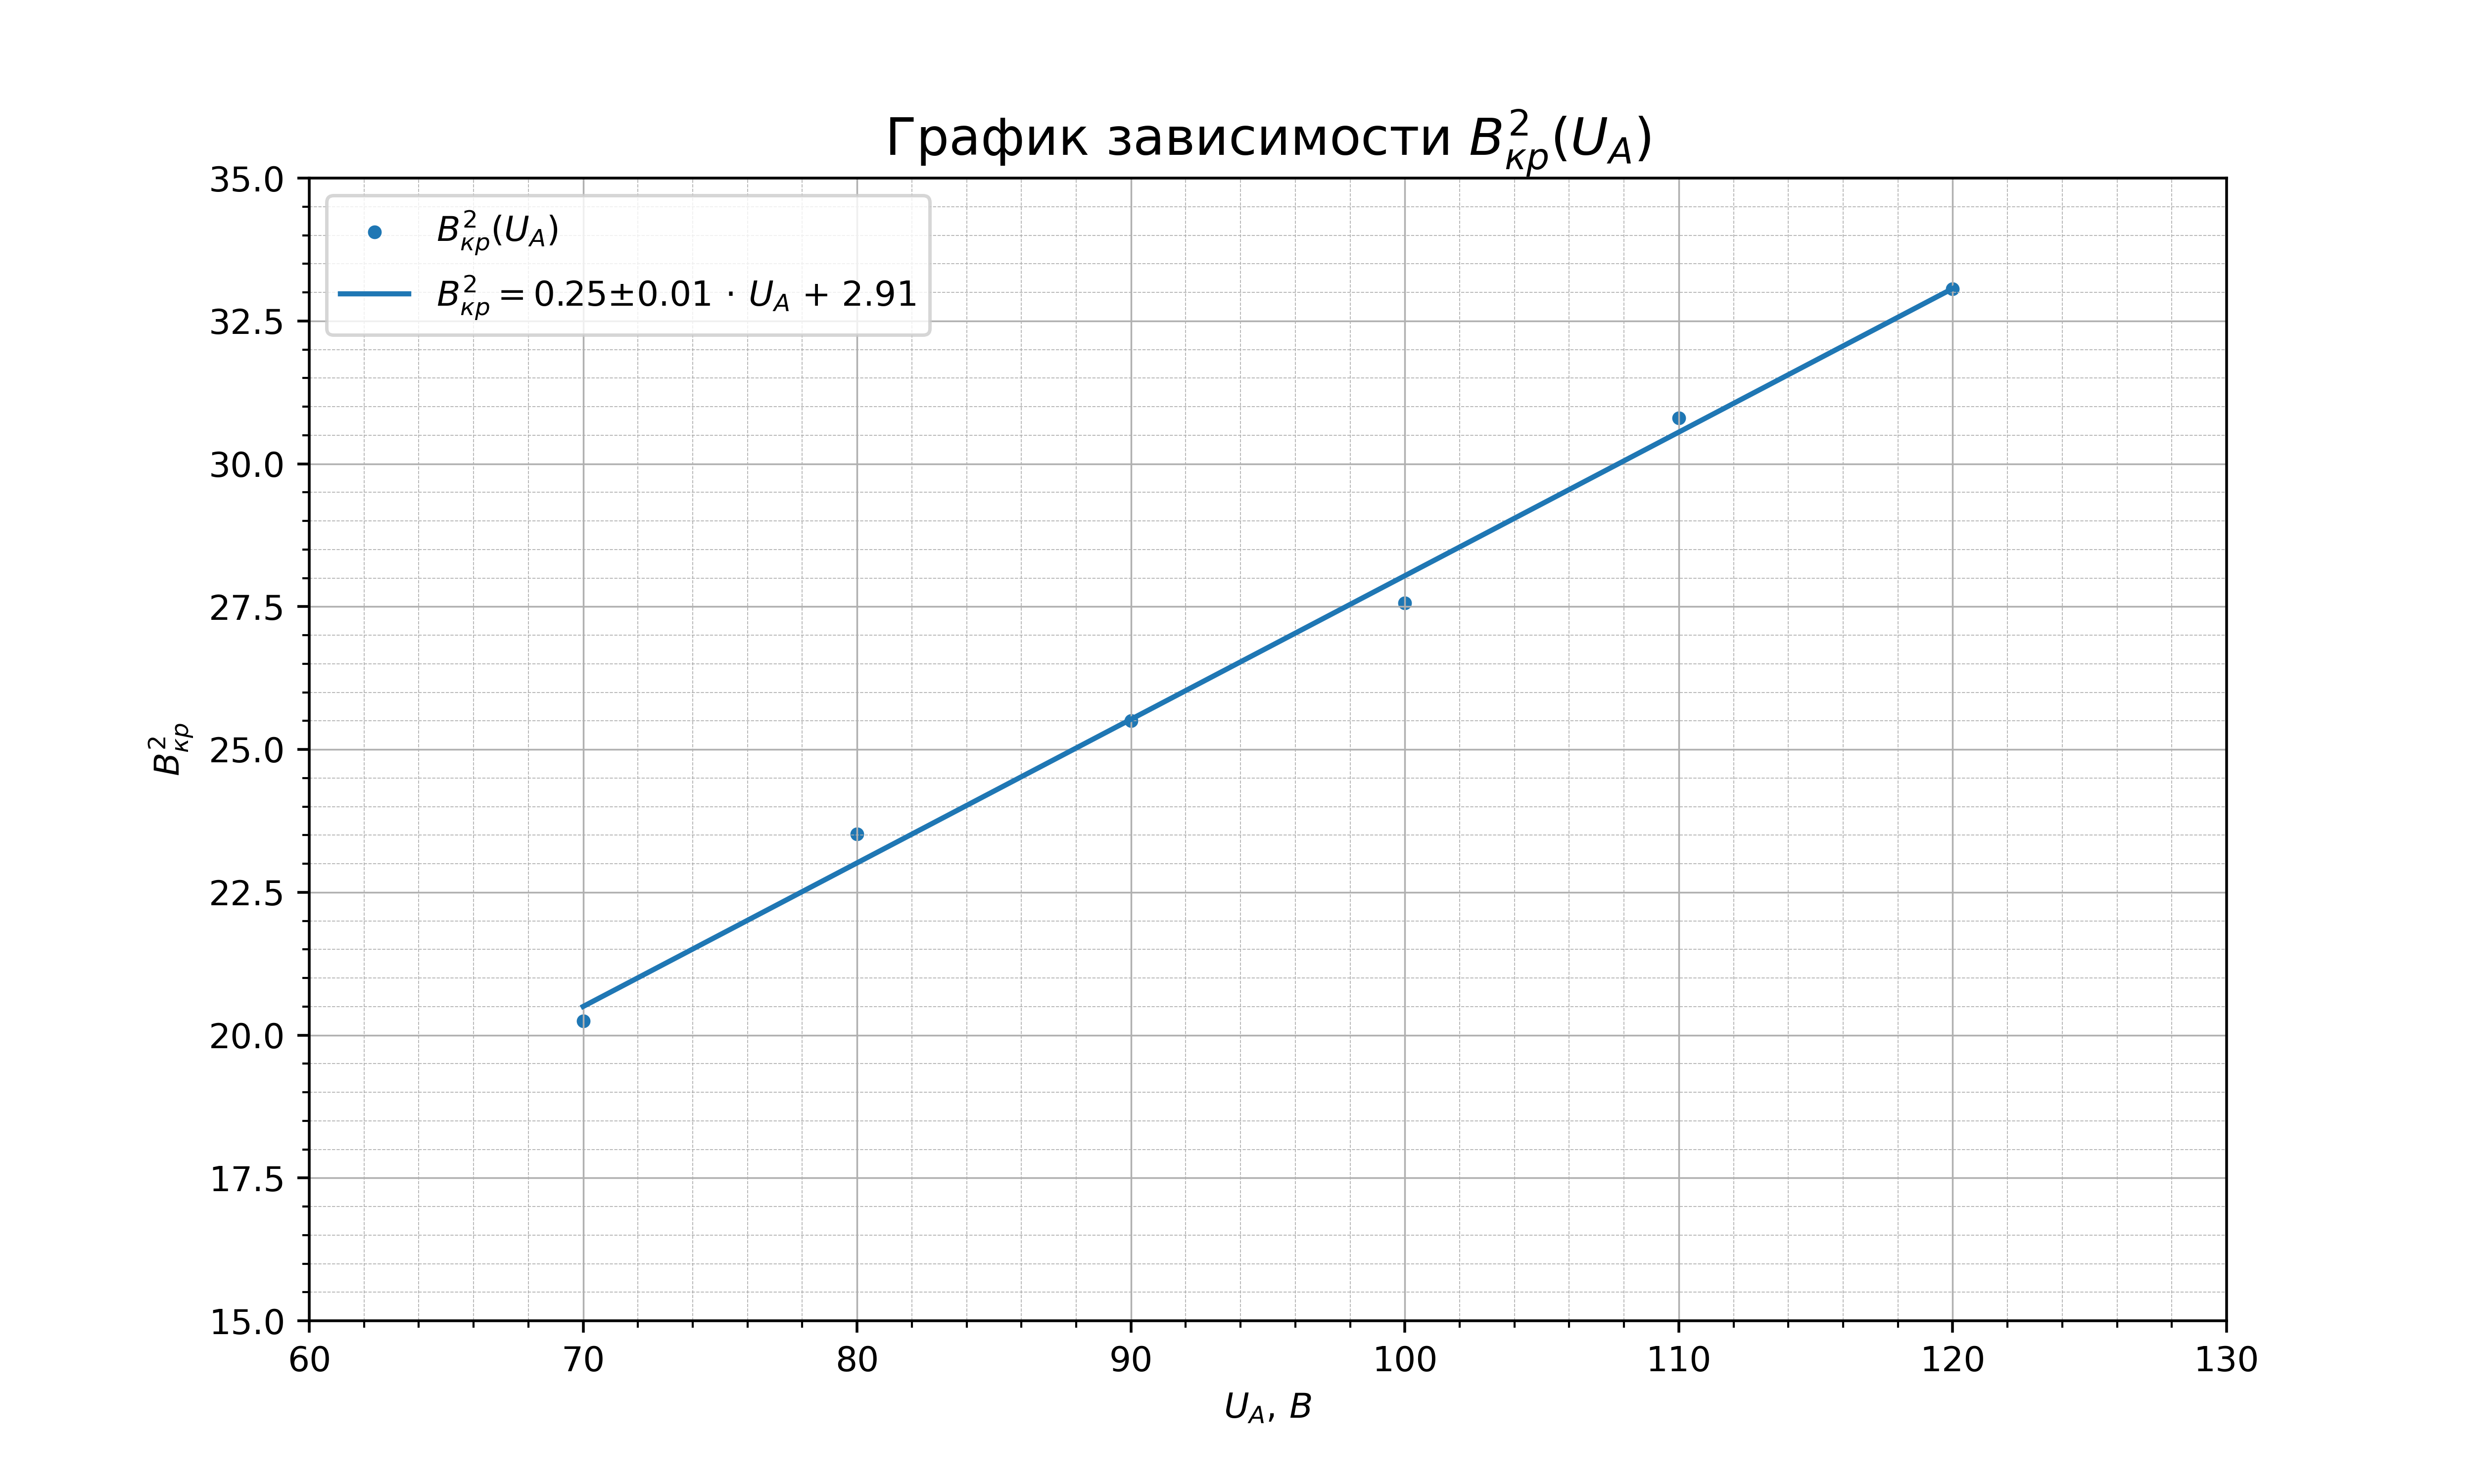
\includegraphics[scale=0.7]{3.3.1_4.png}
\end{flushleft}
\caption{График зависимости $B^2_{кр}(U_A)$}
\label{ris6}
\end{figure}

По формуле \eqref{eq2} вычисляем $e/m$. Полученное значение: $$\frac{e}{m} = 1,9\pm0,1\cdot 10^{11}~Кл/кг.$$

\section{Обсуждение результатов и выводы}

В данной работе был измерен удельный заряд электрона методами магнитной фокусировки и магнетрона. Результаты измерений:

$$\boxed{\begin{aligned}
&1,6\pm0,1\cdot 10^{11}~Кл/кг && \text{--- метод магнитной фокусировки} \\
&1,9\pm0,1\cdot 10^{11}~Кл/кг && \text{--- метод магнетрона} \\
\end{aligned}}$$

Полученные результаты согласуются в пределах погрешности с табличным значением~---~$1,76 \cdot 10^{11}~Кл/кг$. В методе магнитной фокусировки основной вклад в погрешность вносит погрешность определения коэффициента зависимости $B_ф(n)$. Вероятно, при более точной настройки фокусировки осциллографа можно более точно определить точки фокуса. В методе магнетрона основным источником погрешности является погрешность определения $B_{кр}$, так как низкая чувствительность амперметров не позволяет получить достаточно точек на кривой падения $I_A$ и хорошо промерить эту зависимость. При использовании более чувствительных измерительных приборов можно получить больше точек на этой кривой и, следовательно,точнее определить точки $B_{кр}$.

\end{document}